\section{Charged Particle Motion, Radiation}
Last class, we derived the Lorentz force:
\begin{equation}
    \dod{\v{p}}{t} = m\dod{\gamma \v{v}}{t} = q(\v{E} + \v{v} \times \v{B})
\end{equation}
and in the case where $\v{B} = \v{0}, \v{E} = E\xhat$ (and $\v{x}(t=0) = \dot{\v{x}}(t=0) = 0$) we found:
\begin{equation}
    \v{x}(t) = \frac{mc^2}{qE}\left(\sqrt{1 + \left(\frac{qEt}{mc}\right)^2} - 1\right)\xhat, \quad \v{v}(t) = \frac{\frac{qEt}{m}}{\sqrt{1 + \left(\frac{qEt}{mc}\right)^2}}\xhat
\end{equation}

\subsection{Cyclotron motion}
We now consider the case where $\v{E} = 0, \v{B} = B\zhat$, where $\v{x}(t=0) =0$ and $\dot{\v{x}}(t=0) = v_0\xhat$.

The equation of motion is:
\begin{equation}
    \dod{(\gamma \v{v})}{t} = \frac{q}{m}\v{v}\times\v{B}
\end{equation}
Since there are no forces in $\zhat$ the interesting motion is in $xy$. Further, we observe that $\abs{\v{v}}$ is constant, as:
\begin{equation}
    \dod{}{t}((\gamma \v{v}) \cdot (\gamma \v{v})) = \frac{2q}{m}\gamma \v{v} \times (\v{v} \times \v{B}) = 0
\end{equation}
Thus $\gamma^2 v^2$, and therefore $v$ is constant. The solutions to the EOM are:
\begin{equation}
    x(t) = x_0 + R_g\cos(\omega_g t + \phi_0)
\end{equation}
\begin{equation}
    y(t) = y_0 - R_g\sin(\omega_g t + \phi_0)
\end{equation}
\begin{equation}
    z(t) = z_0 + v_0^z t
\end{equation}
where:
\begin{equation}
    \omega_g = \frac{qB}{\gamma m}
\end{equation}
is the cyclotron frequency, and:
\begin{equation}
    R_g = \frac{v}{\abs{\omega_g}}
\end{equation}
is the Larmor radius.

You've likely see this already in your quantum mechanics and classical mechanics courses. But there is one different in the discussion. Usually, when we discuss the quantum (or classical) Hall effect, we never think about the electron moving close to the speed of light (in which case $\gamma \approx 1$) so you've seen $\omega_g \sim \frac{qB}{m}$. But in many situations, e.g. accelerators, $\gamma$ is not small, and so the cyclotron frequency has this important additional factor.

\subsection{Motivation - Radiation of Moving Charges}
In both of the given examples, we have charges that are moving, and moreover, accelerating! Hence we have that these charges emit radiation. We'll go through a lot of technical details to derive the radiation, but before we do that, let's give some motivation for why the detail will be worthwhile.

\begin{center}
    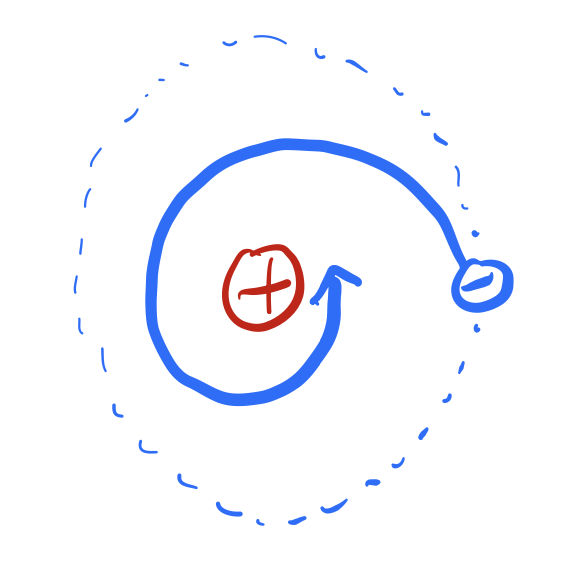
\includegraphics[scale=0.4]{Lectures/Images/lec8-hydrogen.png}
\end{center}

For example, consider a hydrogen atom. In the classical picture, the electron orbits the proton. It then spirals into the proton as it emits radiation (from the effect that we calculate today), and the atom collapses\footnote{And we would be out of drinking water}. But in reality this (fortunately) does not happen, and this is because the radiation emitted from hydrogen atoms are quantized/not continuous. This was one of the confusions of classical physics and was one of the motivations for the development of quantum mechanics.

\begin{center}
    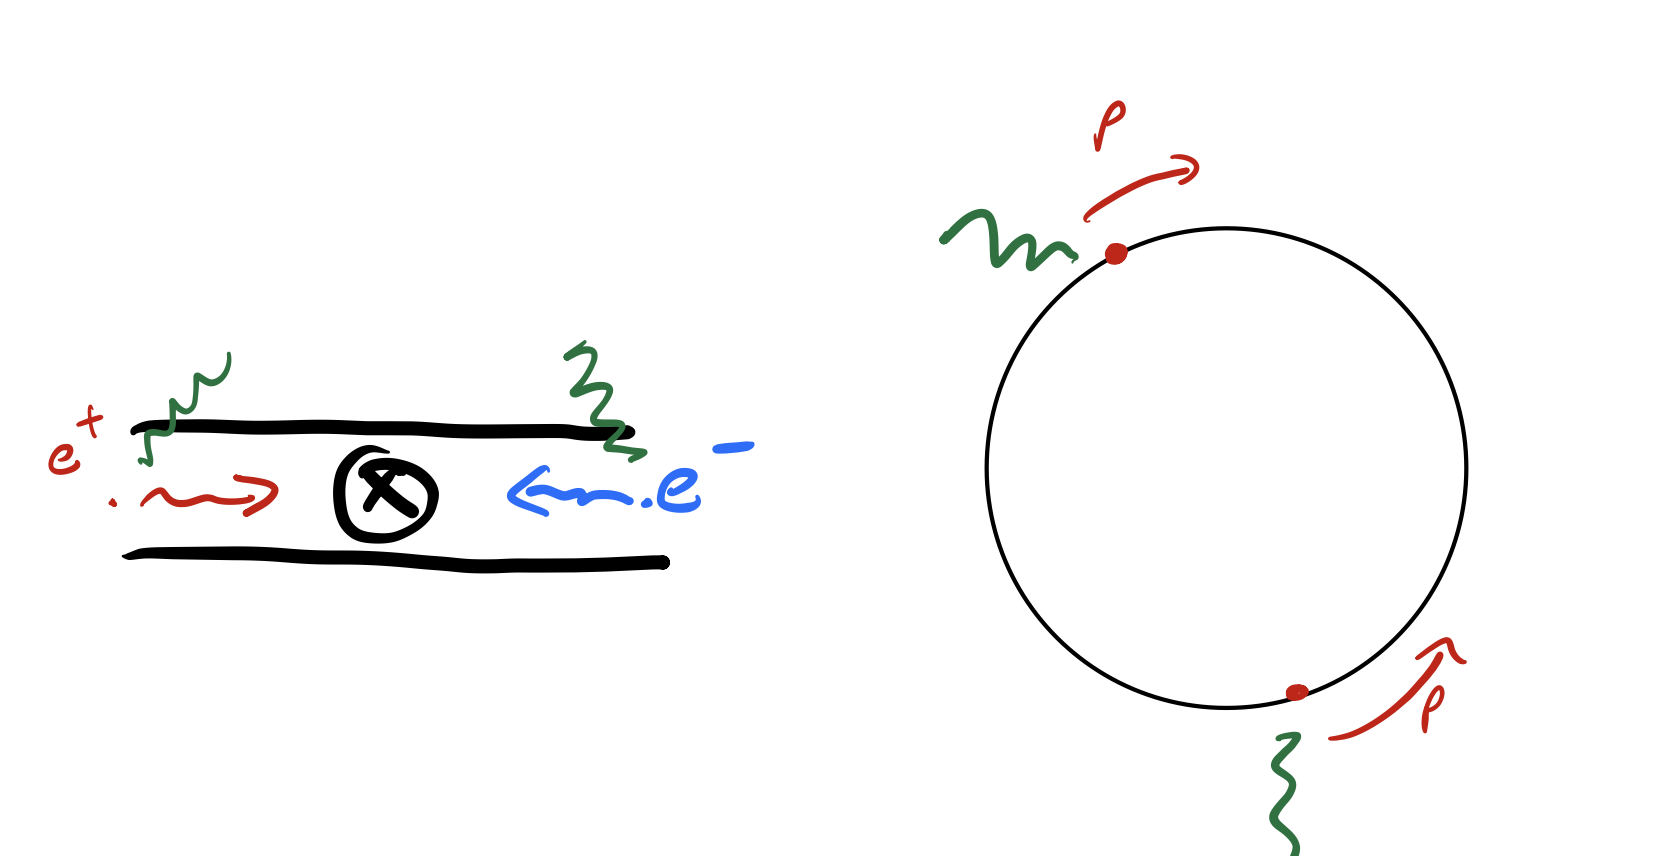
\includegraphics[scale=0.4]{Lectures/Images/lec8-radiation.png}
\end{center}

Another practical example of relevance is accelerators; in either linear or circular accelerators, the accelerating protons/positrons/electrons emit radiation. This is something you have to account for both from an energy efficiency perspective, and also to account for in your signal/measurements as known physics.

\subsection{Calculating fields from charges/currents}
In the last quarter, you saw tha the gauge fields ($\phi, \v{A})$ created by $(\rho, \v{J})$ are given by:
\begin{equation}
    \phi(t, \v{x}) = \frac{1}{4\pi\e_0}\left.\int \frac{d^3\v{x}'}{\abs{\v{x} - \v{x}'}}\rho(t', x')\right|_{\text{ret}}
\end{equation}
\begin{equation}
    \v{A}(t, \v{x}) = \frac{\mu_0}{4\pi}\left.\int \frac{d^3\v{x}'}{\abs{\v{x} - \v{x}'}}\v{J}(t', \v{x}')\right|_{\text{ret}}
\end{equation}

\begin{center}
    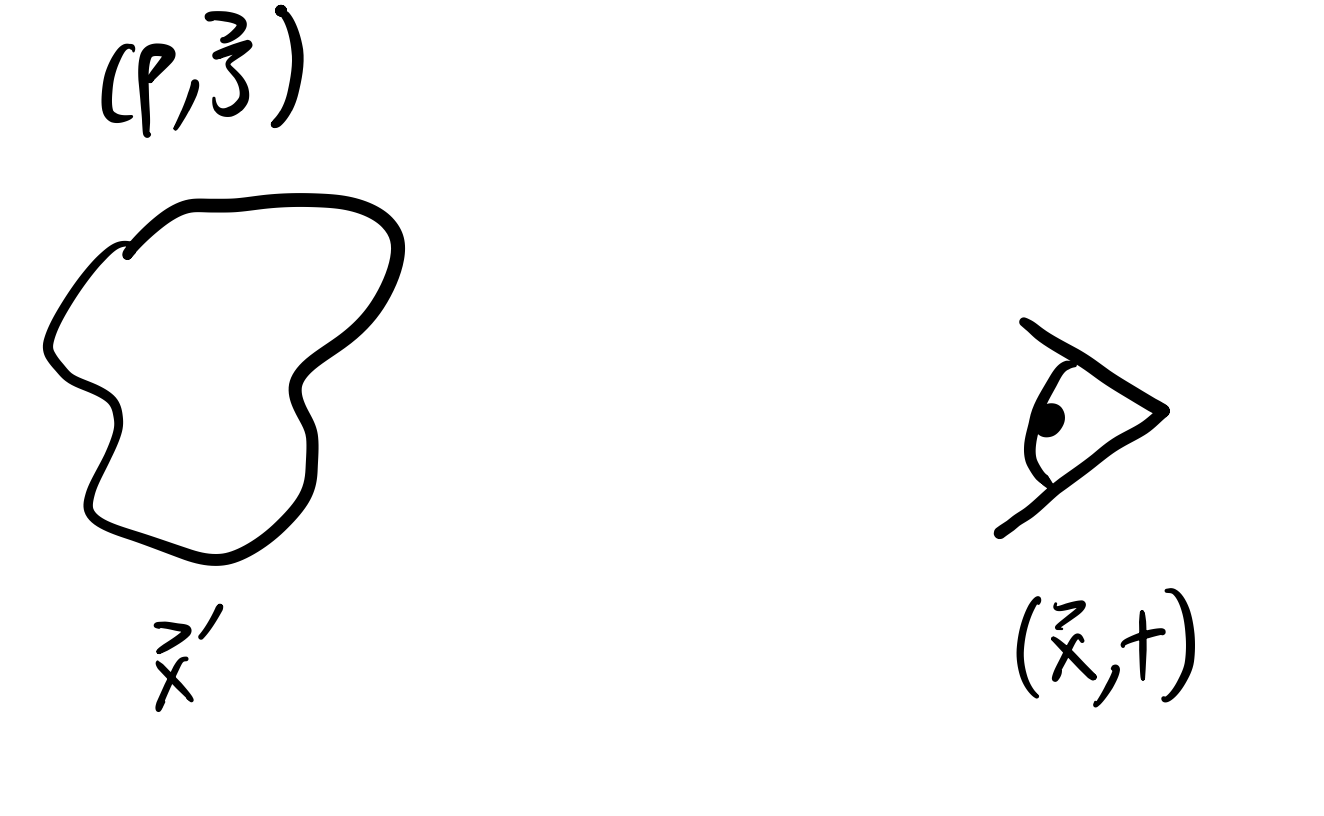
\includegraphics[scale=0.4]{Lectures/Images/lec8-fields.png}
\end{center}

What do these formulas actually say? We integrate over charges/currents at $\v{x}'$, while our location is $\v{x}$ - we evaluate at the retarded time:
\begin{equation}
    t_{\text{ret}} = t' =  t - \frac{1}{c}\abs{\v{x} - \v{x}'}
\end{equation}
which accounts for the locality of the physics - if we move the sources, it takes time for the signal to reach the point $\v{x}$, as the signal is bounded by the speed of light (c.f. the Coloumb force law which acts at a distance).

In terms of the $A_\mu = (-\frac{\phi}{c}, \v{A})$ four vector, we can summarize the above equations as a single one:
\begin{equation}
    A_\mu(t, \v{x}) = \left.\frac{\mu_0}{4\pi}\int \frac{d^3\v{x}'}{\abs{\v{x} - \v{x}'}}J_\mu(t', \v{x}')\right|_{\text{ret}}
\end{equation}

\subsection{Deriving the Leonard-Wiechart Potentials}
Now, we are interested in finding $A_\mu$ for a charged particle is travelling with trajectory $\v{r}(t)$. The charge/current densities are:
\begin{equation}
    \rho(t, \v{x}) = q\delta(\v{x} - \v{r}(t))
\end{equation}
\begin{equation}
    \v{J}(t, \v{x}) = q\dot{\v{r}}\delta(\v{x} - \v{r}(t))
\end{equation}
So we can calculate:
\begin{equation}
    \phi(t, \v{x}) = \frac{q\mu_0 c^2}{4\pi^2}\int \frac{d^3\v{x}'}{\abs{\v{x} - \v{x}'}}\delta(\v{x}' - \v{r}(t_{\text{ret}}))
\end{equation}
\begin{equation}
    \v{A}(t, \v{x}) = \frac{q\mu_0}{4\pi}\int \frac{d^3\v{x}'}{\abs{\v{x} - \v{x}'}}\dot{\v{r}}(t_{\text{ret}})\delta(\v{x}' - \v{r}(t_{\text{ret}}))
\end{equation}
Usually, we would say that the integral of a delta function is quite easy, but here there is a slight complication. The problem is that $\v{r}(t_{\text{ret}})$ depends on $\v{x}'$ through $t_{\text{ret}}$:
\begin{equation}
    \v{t}(t_{\text{ret}}) = \v{r}(t - \frac{1}{c}\abs{\v{x} - \v{x}'})
\end{equation}

To resolve this, let us study the 1-D analog, where we recall the delta function identity:
\begin{equation}
    \int dx g(x) \delta(f(x))  = \left.\frac{g}{\abs{f'}}\right|_{f'=0}
\end{equation}
In 3-D:
\begin{equation}
    \begin{split}
        \int d^3\v{x}g(\v{x})\delta(\v{f}(\v{x})) &= \int d^3\v{x}g(\v{x})\delta(f_1(\v{x}))\delta(f_2(\v{x}))\delta(f_3(\v{x}))
        \\ &= \left.\frac{g}{\abs{J}}\right|_{\v{f}(\v{x}) = 0}
    \end{split}
\end{equation}
where $J$ is the 3x3 matrix:
\begin{equation}
    J^i_{j} = \ddpd{f^i}{x^j}
\end{equation}
and $\abs{J} = \det J$.

With that mathematical aside, let's turn back to our problem. We have:
\begin{equation}
    g(\v{x}) = \frac{1}{\abs{\v{x} - \v{x}'}}
\end{equation}
and:
\begin{equation}
    \v{f}(\v{x}') = \v{x}' - \v{r}(t_{\text{ret}}) = \v{x}' - \v{r}(t - \frac{1}{c}\abs{\v{x} - \v{x}'})
\end{equation}
Calculating $J$\footnote{Kutasov: ``The location of indices are important if you are doing mechanics from Arnold's textbook. If you choose not to subscribe to this, I support you in this decision - they are not that important. Wald may care about this - he may worship at the altar of Arnold, but not me''}:
\begin{equation}
    J^i_j = \ddpd{f^i}{x'^j} = \delta^j_i - \frac{x^j - x'^j}{c\abs{\v{x} - \v{x}'}}\left.\dod{r^i}{t}\right|_{t_\text{ret}}
\end{equation}
To eleborate on this slightly:
\begin{equation}
    \ddpd{}{x'^j}\abs{\v{x} - \v{x}'} = \ddpd{}{x'^j}\left((x_1 - x_1')^2+ (x_2 - x_2')^2 + (x_3 - x_3')^2\right)^{1/2} = \frac{1}{2}\frac{(-1)}{\abs{\v{x} - \v{x}'}}2(x_j - x_j')
\end{equation}
and the full expression we get from that and the chain rule. Evaluating the determinant:
\begin{equation}
    J = \abs{-\frac{\v{x} - \v{x}'}{c\abs{\v{x} - \v{x}'}}\left.\dod{\v{r}}{t}\right|_{t_\text{ret}}}
\end{equation}
Now, if we use this result to evaluate the potentials, we get the Leonard-Wiechart potentials:
\begin{equation}
    \phi(t, \v{x}) = \frac{\mu_0 c^2}{4\pi}\frac{1}{\alpha}\frac{q}{\abs{\v{x} - \v{r}(t_{\text{ret}})}}
\end{equation}
\begin{equation}
    \v{A}(t, \v{x}) = \frac{\mu_0}{4\pi}\frac{1}{\alpha}\frac{q}{\abs{\v{x} - \v{r}(t_{\text{ret}})}}\left.\dod{\v{r}}{t}\right|_{t_\text{ret}}
\end{equation}
Where:
\begin{equation}
    \alpha = 1 -\frac{1}{c}\hat{\v{n}}\cdot \left.\dod{\v{r}}{t}\right|_{t_\text{ret}}
\end{equation}
and:
\begin{equation}
    \hat{\v{n}} = \frac{\v{x} - \v{r}(t_{\text{ret}})}{\abs{\v{x} - \v{r}(t_{\text{ret}})}}
\end{equation}
is the direction from the point we are evaluating the potentials $\v{x}$ to where the particle \emph{was} when we see the signal, assuming the signal travels at the speed of light (hence the evaluation at the retarded time). $t_{\text{ret}}$ implicitly depends on $\v{r}(t_{\text{ret}})$:
\begin{equation}
    t_{\text{ret}} = t - \frac{1}{c}\abs{\v{x} - \v{r}(t_{\text{ret}})}
\end{equation}
and thus solving for this implicitly is the first step of using these potentials. This looks all complicated, but it is all in service of making sure that we do not have action at a distance - physics is local, and it takes time for information to propagate. This hopefully makes the retarded time at least conceptually intuitive.

\begin{center}
    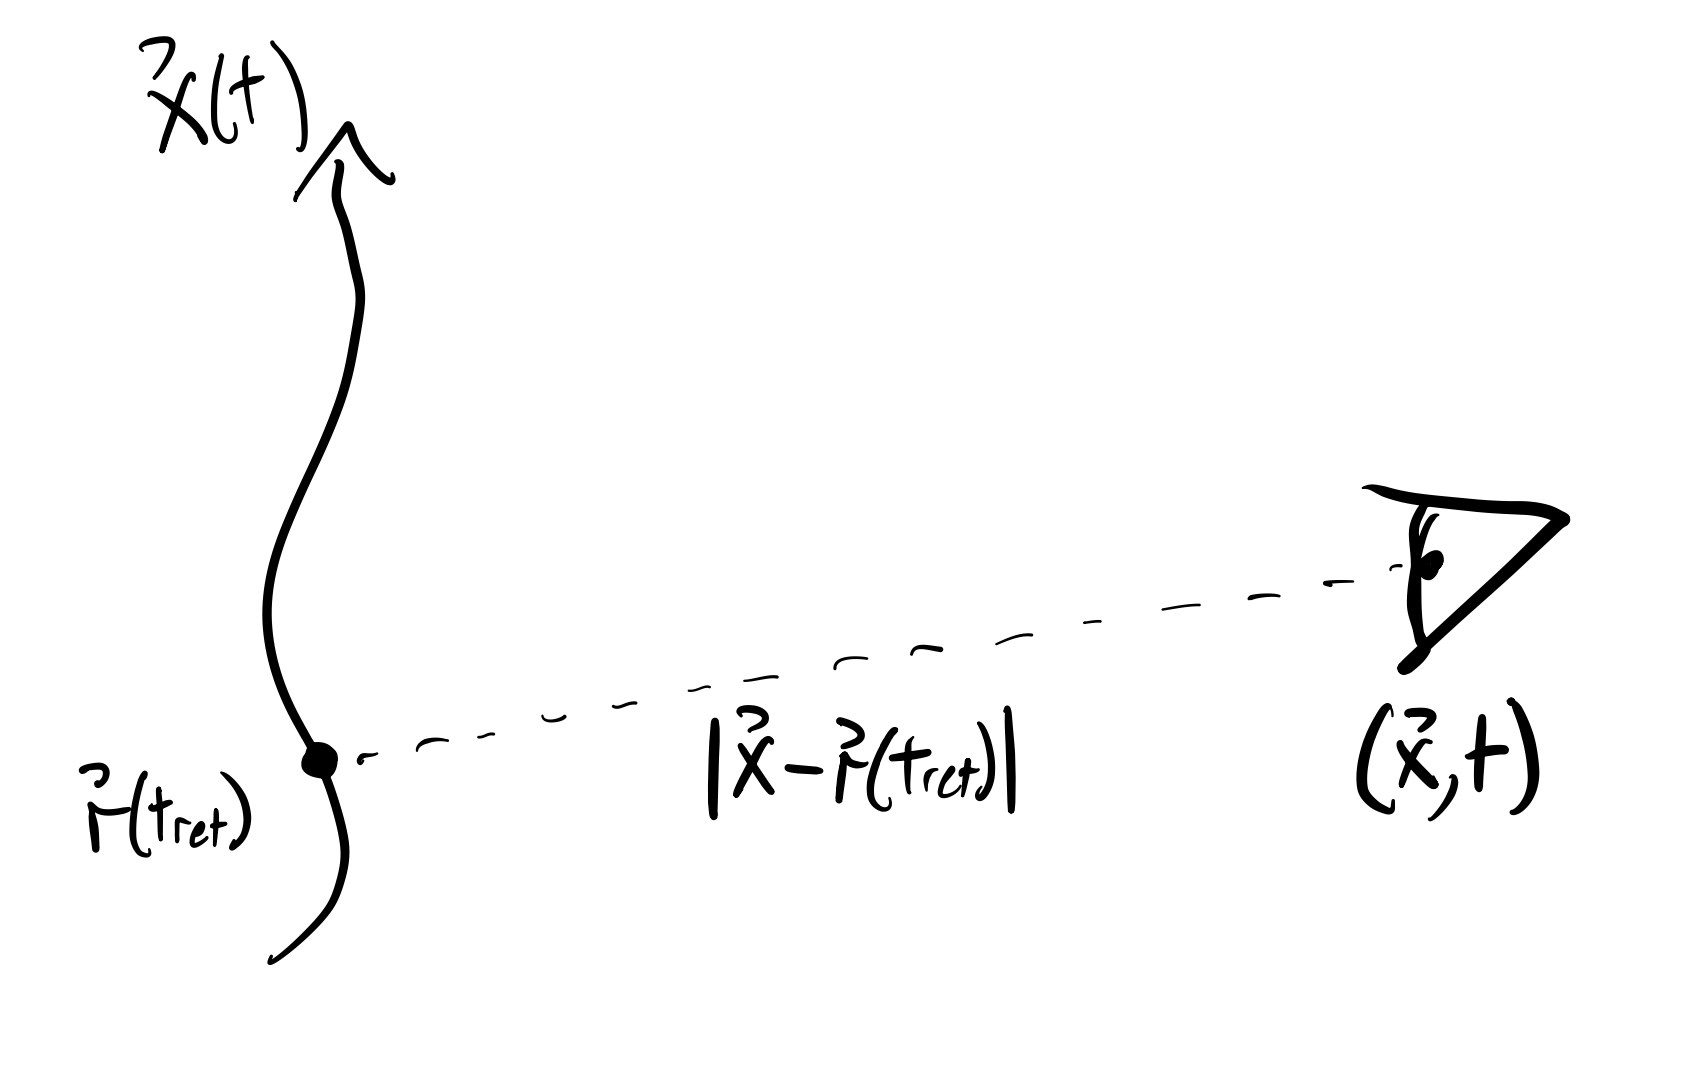
\includegraphics[scale=0.4]{Lectures/Images/lec8-retardedtime.png}
\end{center}

\subsection{Coloumb's Law}
Let $\v{r}(t) = \v{r}_{\text{particle}}$ be a constant/fixed position in space for a particle of charged $q$. Then, we find that $\alpha = 1$, and we get for the potentials:
\begin{equation}
    \phi(t, \v{x}) = \frac{\mu_0 c^2}{4\pi}\frac{q}{\abs{\v{x} - \v{r}_{\text{particle}}}}
\end{equation}
\begin{equation}
    \v{A} = 0
\end{equation}
which is consistent with Coloumb's law. All of the retarded time parts of the expression drops out. But in the case that the particle is accelerating, e.g. we turn on some electric field, the retarded time becomes very important - because we don't see what the particle is doing \emph{now}, but what it was doing some time ago.

\subsection{E/B fields from Leonard-Wiechart Potentials}

We can further ask - what are the $\v{E}, \v{B}$ fields? Normally you could say - look, we have the $A_\mu$, now give it to the graduate student to calculate the fields, but alas you are the graduate students so we must do it. Recall:
\begin{equation}
    \v{E} = -\nabla \phi - \dot{\v{A}}
\end{equation}
\begin{equation}
    \v{B} = \nabla \times \v{A}
\end{equation}
In $\v{E}$ we see the time derivative appear, and so to calculate this we must know:
\begin{equation}
    \dpd{t_{\text{ret}}}{t} = \frac{1}{\alpha}
\end{equation}
you can work through this yourself, see Wald, or see Kutasov's notes for why this is the case. We also will need:
\begin{equation}
    \nabla t_{\text{ret}} = -\frac{1}{\alpha}\hat{\v{n}}
\end{equation}

Now, if we plug in $\phi, \v{A}$ into the expressions for $\v{E}, \v{B}$, we obtain:
\begin{equation}
    \v{E}(t, \v{x}) = q\frac{\mu_0 c^2}{4\pi}\frac{(\hat{\v{n}} - \frac{1}{c}\dod{\v{r}}{t})(1 - \frac{1}{c^2}\left(\dod{\v{r}}{t}\right)^2)}{\alpha^3\abs{\v{x} - \v{r}(t_{\text{ret}})}^2} + q\frac{\mu_0}{4\pi}\frac{\hat{\v{n}} \times [(\hat{\v{n}} - \frac{1}{c}\dod{\v{r}}{t})\times \dod[2]{\v{r}}{t}]}{\alpha^3\abs{\v{x} - \v{r}(t_{\text{ret}})}}
\end{equation}
where all time derivatives are evaluated at the retarded time. The expression for the magnetic field is comparively simple.
\begin{equation}
    \v{B}(t, \v{x}) = \hat{\v{n}} \times \v{E}
\end{equation}

and we will analyze these next time - in particular, from the exact expressions above, we will study the radiation we see at spatial infinity. To this end, the first term will not be so important because it is $\frac{1}{x^2}$ (as opposed to the $O(\frac{1}{x})$ term). The first term in $\v{E}$ corresponds to the Coloumb force, the second term (which depends on the acceleration of the particle! key for radiation) gives us a Poynting vector that goes as $O(\frac{1}{x^2})$.